\documentclass[11pt,a4paper]{article}
\usepackage[margin=2.2cm]{geometry}
\usepackage{fontspec}
\setmainfont{TeX Gyre Pagella}
\setmonofont{DejaVu Sans Mono}[Scale=0.82]
\usepackage{amsmath,amssymb,amsthm}
\usepackage{graphicx,xcolor,listings,booktabs,enumitem}
\usepackage[most]{tcolorbox}
\usepackage[hidelinks]{hyperref}

\definecolor{accent}{HTML}{2B6CB0}
\definecolor{warn}{HTML}{C53030}
\newtcolorbox{keybox}[1][]{colback=accent!5,colframe=accent,boxrule=0.6pt,arc=2pt,left=6pt,right=6pt,top=4pt,bottom=4pt,#1}
\newtcolorbox{warnbox}{colback=warn!5,colframe=warn,boxrule=0.6pt,arc=2pt,left=6pt,right=6pt}

\lstdefinelanguage{Rust}{
  keywords={fn,let,mut,if,else,for,in,while,return,use,pub,struct,impl,loop,break,Some,None,as,match,const},
  morekeywords=[2]{usize,i32,u64,f64,bool,Vec,VecDeque,BTreeSet,BinaryHeap,Option},
  sensitive=true, morecomment=[l]{//}, morestring=[b]"}
\lstset{language=Rust,basicstyle=\ttfamily,keywordstyle=\color{accent}\bfseries,
  keywordstyle=[2]\color{teal},commentstyle=\color{gray}\itshape,stringstyle=\color{warn},
  frame=single,rulecolor=\color{gray!40},backgroundcolor=\color{gray!4},
  numbers=left,numberstyle=\tiny\color{gray},xleftmargin=1.5em,breaklines=true,
  columns=fullflexible,keepspaces=true,showstringspaces=false}

\newtheorem*{invariant}{Invariant}
\theoremstyle{definition}\newtheorem*{definition}{Definition}


\newcommand{\board}[2]{\begin{center}\fcolorbox{gray!50}{white}{\includegraphics[width=#1]{board/#2.jpg}}\end{center}}
\newcommand{\profpage}[3]{\begin{center}\fcolorbox{gray!50}{white}{\includegraphics[page=#2,width=#1,trim=0 #3 0 0,clip]{SlidingWindowMaxima.pdf}}\\[-2pt]{\footnotesize\textcolor{gray}{Prof.'s notes, \texttt{SlidingWindowMaxima.pdf} p.\,#2}}\end{center}}
\newcommand{\extra}{\textsuperscript{\textcolor{warn}{[extra]}}}

\title{\textbf{CPC --- Lecture 3}\\[2pt]\large Sliding Window Maxima in linear time, Trapping Rain Water,\\ the 100 Prisoners Puzzle}
\author{Competitive Programming and Contests --- Wednesday 23/09/2026}
\date{}

\begin{document}
\maketitle
\vspace{-1.5em}
\begin{keybox}
\textbf{Sources.} Recording \texttt{L\_03.mp4} (1h43m): automatic transcript + frames of the professor's
iPad notes (the handwritten images in this document are \emph{his} board).
The professor's notebook for this part (\texttt{SlidingWindowMaxima.pdf}, 11 pages: Trapping Rain Water, SWM from L2 to L3,
``is a binary tree a BST?'') is in this folder; its pages replace the video frames where they cover the same content.
Rust code of the SWM: Prof.\ Rossano's note \url{https://pages.di.unipi.it/rossano/blog/2023/swm/}.
Parts marked \extra{} are \emph{not} from the lecture (my additions: plots, proofs completed, code).
\end{keybox}

\noindent Code: \texttt{Lessons/L3/src/lib.rs} --- \texttt{cargo test -p l3},
\texttt{cargo run -p l3 --release --bin swm}, \texttt{cargo run -p l3 --release --bin prisoners}.

\tableofcontents

%======================================================================
\section{Recap of L2 and the method}
\begin{itemize}[nosep]
\item Trivial solution $\Theta(nk)$: each window is recomputed from scratch although only one element enters and one leaves.
\item Each step needs three operations on a \emph{multiset} (the window): \textbf{remove} an element, \textbf{insert} an element, \textbf{report the max}.
      The trivial solution is just a trivial data structure for them.
\item \textbf{Heap + lazy delete}: store pairs $\langle$value, position$\rangle$; remove an element only when it is the max and lies outside the window.
      $\#\text{insertions}=n$, $\#\text{extractions}\le n$ (each element removed at most once) $\Rightarrow \Theta(n\log n)$.
      \emph{``Being lazy is something we are going to do often, because it simplifies things.''}
\item \textbf{BST} (predecessor problem: insert, delete, search, min/max, successor, predecessor in $\Theta(\log|S|)$) storing only the window $\Rightarrow \Theta(n\log k)$.
\end{itemize}
\begin{keybox}
\textbf{Method:} trivial solution $\to$ isolate the operations it needs $\to$ find a data structure supporting them.
$\Theta(n\log k)$ is enough in most practical cases (and probably in interviews), but it is not optimal: the optimum is $\Theta(n)$,
since the whole array must be read at least once.
\end{keybox}

%======================================================================
\section{Sliding Window Maxima in $\Theta(n)$}

\subsection{The deque, and how it is implemented}
A \textbf{deque} (double-ended queue) allows access, insertion and deletion at both \textbf{head} and \textbf{tail} in $O(1)$ (amortized).
Every language has one (Rust: \texttt{VecDeque}). Possible implementations:
\begin{itemize}[nosep]
\item \textbf{circular array} with a head and a tail pointer --- requires knowing the maximum size in advance;
\item \textbf{linked list} --- works in $O(1)$ for these operations, but ``in real life nobody uses a list''. Four inefficiencies:
  \begin{enumerate}[nosep]
  \item an allocation/deallocation for every insertion/deletion (expensive);
  \item scanning is cache-unfriendly (you jump around memory), while scanning an array is very fast;
  \item no random access;
  \item extra space for the pointers: with small keys you roughly double the space.
  \end{enumerate}
  (Python ``lists'' are actually arrays.)
\item \textbf{list of blocks}: each node is a fixed-size block of elements. Allocations only when a block is full/empty, jumps during a scan
      are only $\#\text{elements}/\text{block size}$, and the pointer cost is amortized over the block. This is how deques are usually implemented.
\end{itemize}

\subsection{Algorithm}
Keep a deque $Q$ of pairs $\langle e,p\rangle$ (value, position) --- the position tells us whether an element is still in the window.
\profpage{0.62\linewidth}{9}{0bp}
Repeat $n$ times:
\begin{enumerate}[nosep]
\item move the window one position to the right; let $y$ be the new element;
\item \textbf{head}: remove from the head of $Q$ the elements outside the window; \textbf{stop} as soon as the current head is inside the window
      (lazy: elements outside the window may remain in the middle of $Q$, we don't scan it all);
\item \textbf{tail}: insert $y$ from the tail, removing every element $\le y$; \textbf{stop} as soon as the tail is $>y$;
\item report the head of $Q$ as the max of the window.
\end{enumerate}

\noindent Intuition example from the board: window = positions $10..15$, new element $11$ at position 15.
From the head, $\langle 42,8\rangle$ and $\langle 40,9\rangle$ are outside $\Rightarrow$ removed; $\langle 38,11\rangle$ is inside $\Rightarrow$ stop
(whatever is in the middle is not touched). From the tail, the elements $\le 11$ are removed, then $\langle 11,15\rangle$ is appended.
\board{0.35\linewidth}{q_example}

\noindent The prof also remarked that such an ``almost English'' description is precise enough to be used directly as a prompt to generate working code.

\subsection{Running example}
Array used in class (modified on the board so that values and positions differ): $A=[1,3,2,1,1,2,4,3,2]$, $k=3$, positions from 1.
The window starts ``before'' the array, so the first $k-1$ reported values refer to partial windows (skip them if you don't consider them valid).
\board{0.7\linewidth}{trace}
Board: $R = 1,3,3,3,2$ (then $2$). Note the step at $p=5$: the new $1$ \emph{kills} the old $\langle1,4\rangle$ because the removal condition is $\le$.
The two final $2$'s are different elements: the first is the max of the window $[2,1,1]$, the second the max of $[1,1,2]$.
\begin{figure}[h]
\centering
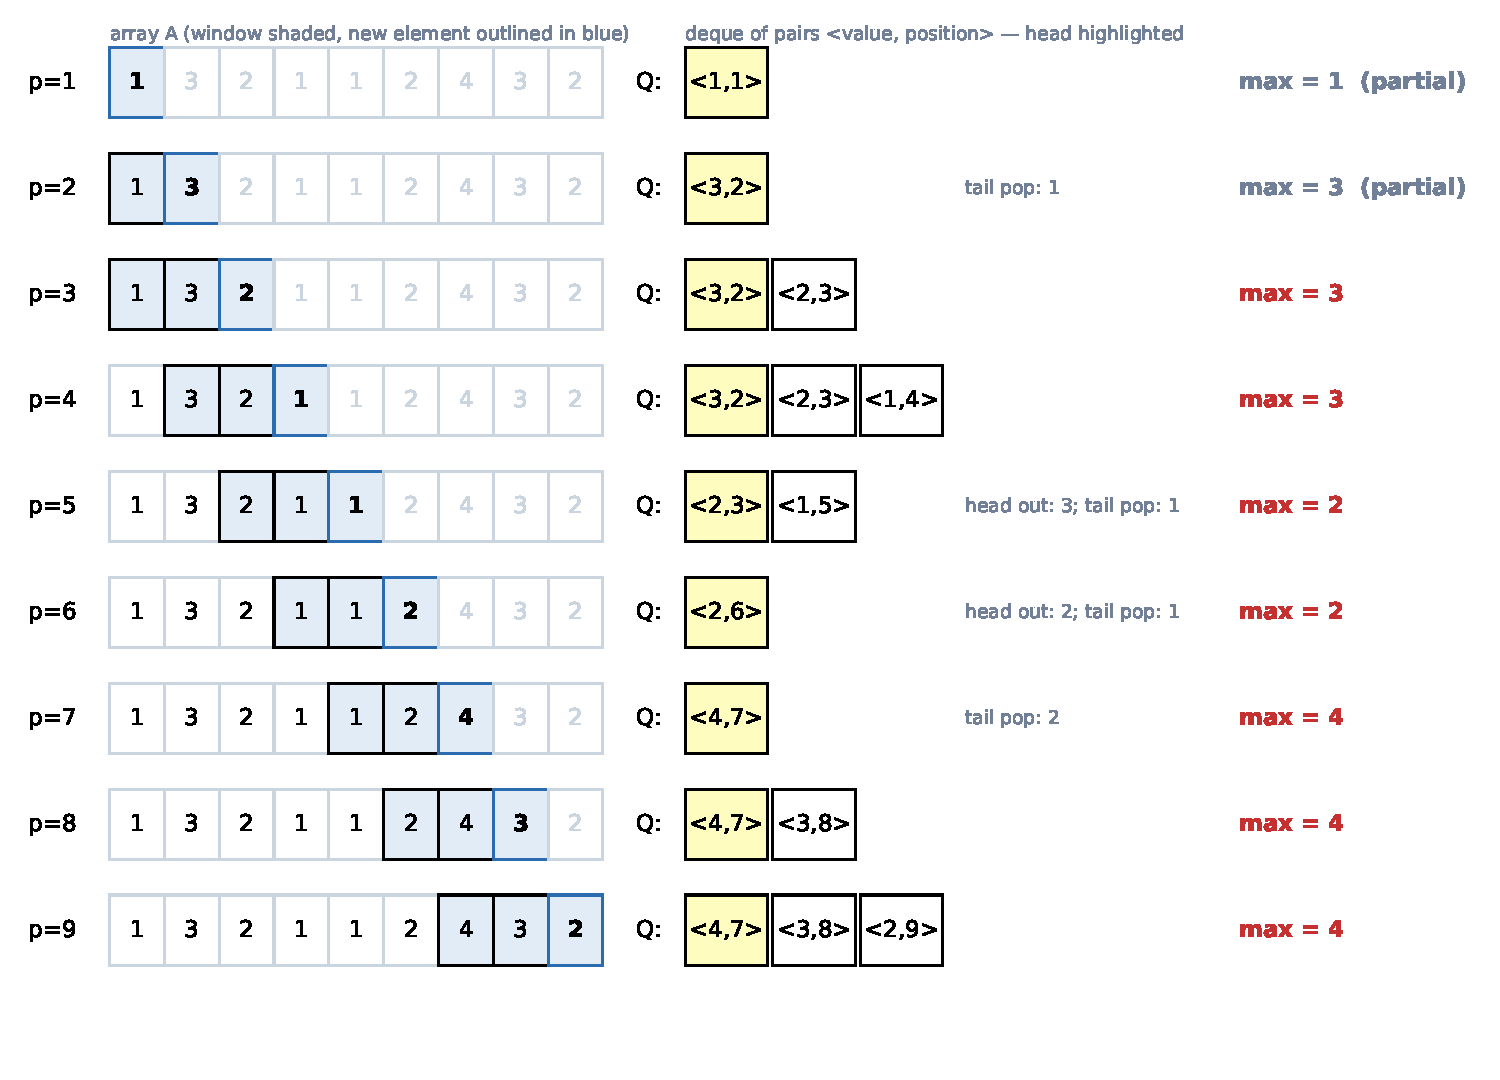
\includegraphics[width=\linewidth]{figs/deque_trace.pdf}
\caption{\extra{} Full trace (the board stopped at $p=6$). Full windows: $3,3,2,2,4,4,4$.}
\end{figure}

\subsection{Time complexity}
Running time $\propto$ \#iterations + \#removals from head + \#removals from tail.
Every element is pushed exactly once and removed at most once (same argument as the lazy heap):
\[
\#\text{removes} + \#\text{pushes} \;\le\; n + n = 2n \text{ operations, each } O(1) \;\Rightarrow\; \Theta(n).
\]

\subsection{Correctness}
\paragraph{Property 1.} $Q$ is sorted in decreasing order.

\noindent\emph{Proof (by contradiction, as in class).} Assume $Q$ is not sorted: then there are two consecutive elements $\langle x,p_x\rangle$ (closer to the head)
and $\langle y,p_y\rangle$ with $x\le y$.
\begin{itemize}[nosep]
\item $p_x>p_y$: in $A$ we have $y$ before $x$. Impossible: insertions happen at the tail, so $x$ (inserted later) would be behind $y$, not before it.
\item $p_x<p_y$: $x$ comes first in $A$. When $y$ was inserted from the tail, it found $x$ immediately above it and, since $x\le y$, it would have killed it.
\end{itemize}
Both cases are impossible $\Rightarrow Q$ is sorted. (A student gave the equivalent inductive argument: each new element stops right below a larger one.) \qed
\profpage{0.6\linewidth}{10}{0bp}

\paragraph{Definition.} An element is a \textbf{right leader} (RL) iff it is greater than any element on its right (in the window).
Example: in $4\,2\,3\,1\,1$ the RLs are $4$, $3$ and the last $1$ (the first $1$ is not: another $1$ follows it; the last element is always an RL).
The maximum of the window is always an RL.

\paragraph{Property 2.} At every iteration $Q$ contains \textbf{all and only} the right leaders of the window.

\noindent\emph{Proof.}
\begin{enumerate}[nosep]
\item \textbf{All}: an RL cannot be killed by any of the next elements, because they are all smaller.
\item \textbf{Only}: the head $a$ is in the window (step 2 of the algorithm). Could there be, further down in $Q$, an element $b$ outside the window?
      Then $b$ comes before $a$ in the array, so the insertion of $a$, which happened after $b$, would have killed $b$ from the tail
      ($b$ is below $a$ in the sorted $Q$, so $b\le a$). \qed
\end{enumerate}
\profpage{0.6\linewidth}{11}{48bp}
\noindent\extra{} The proof in class covers the elements outside the window; for elements \emph{inside} the window that are not RLs:
such an element has a larger (or equal) element to its right, whose later insertion killed it.

\begin{keybox}
The max of the window is an RL $\Rightarrow$ it is in $Q$; $Q$ is sorted $\Rightarrow$ it is the head. The reported element is the maximum.
Note: ``all'' alone would already imply that the maximum is in $Q$ and, since the head is cleaned by step 2, on top.
\end{keybox}

\subsection{Code (Prof.\ Rossano, from the note)}
\begin{lstlisting}
use std::collections::VecDeque;

fn linear(nums: &Vec<i32>, k: usize) -> Vec<i32> {
    let n = nums.len();
    if k > n {
        return Vec::<i32>::new();
    }

    let mut q: VecDeque<usize> = VecDeque::new();
    let mut maxs: Vec<i32> = Vec::with_capacity(n - k + 1);

    for i in 0..k {
        while (!q.is_empty()) && nums[i] > nums[*q.back().unwrap()] {
            q.pop_back();
        }
        q.push_back(i);
    }
    maxs.push(nums[*q.front().unwrap()]);

    for i in k..n {
        while !q.is_empty() && q.front().unwrap() + k <= i {
            q.pop_front();
        }

        while (!q.is_empty()) && nums[i] > nums[*q.back().unwrap()] {
            q.pop_back();
        }
        q.push_back(i);
        maxs.push(nums[*q.front().unwrap()]);
    }
    maxs
}
\end{lstlisting}
\noindent Differences from the board version: the code stores only positions (the value is \texttt{nums[p]}), reports only full windows,
and removes from the tail only elements \emph{strictly} smaller (\texttt{>}), so equal values stay in $Q$ (then $Q$ is non-increasing and may contain
equal non-RLs; still correct, the head is a maximum). The board version (pairs, $\le$, partial windows) is in \texttt{extra::linear\_lecture}\extra.

\paragraph{Exercise suggested by the prof.} Implement all three solutions in Rust (good practice with the standard library: \texttt{BTreeSet}, \texttt{BinaryHeap},
\texttt{VecDeque}) and \textbf{benchmark} them, varying $n$ and $k$ and also on \emph{adversarial} arrays, to see which is fastest in practice.
\extra{} One run of \texttt{cargo run -p l3 --release --bin swm} ($n=10^6$ random values, cloud machine, only indicative):
\begin{center}
\begin{tabular}{lrr}
\toprule
 & $k=10$ & $k=1000$ \\
\midrule
brute force & 10 ms & 394 ms\\
BST & 67 ms & 153 ms\\
heap & 106 ms & 40 ms\\
deque & 14 ms & 19 ms\\
\bottomrule
\end{tabular}
\end{center}
Adversarial ideas to try: an increasing array (the heap never removes anything lazily until the end\,---\,it grows to $n$), a decreasing array (the deque keeps $k$ elements).

\subsection{\extra{} Related exercise: Next Larger Element}
For each $A[i]$, find the first strictly larger element to its right. Same ``kill the dominated elements'' idea with a stack of positions
waiting for their answer: when $A[i]$ arrives it is the answer for every smaller element on top of the stack. $\Theta(n)$ (\texttt{extra::next\_larger}).

%======================================================================
\section{Trapping Rain Water}
\subsection{Problem}
The second problem of L1. An array $H$ is an elevation map: $H[i]$ is the height of a wall at position $i$. It rains; how many unit squares of water are trapped?
Example from class: $H=[6,2,0,4,0,1,0,5,0,3]$.
\begin{figure}[h]
\centering
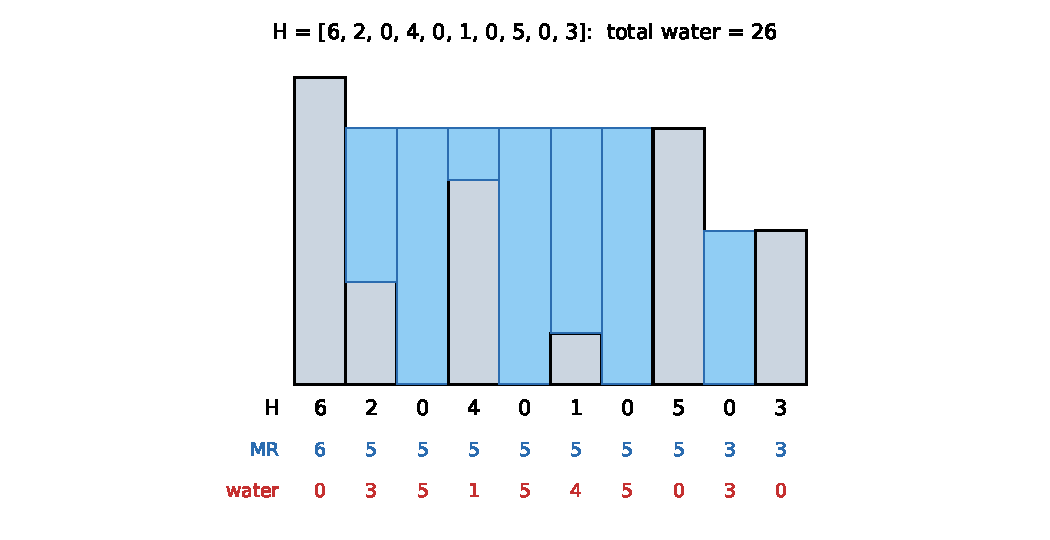
\includegraphics[width=0.75\linewidth]{figs/trw.pdf}
\caption{\extra{} The example with the trapped water; total $26$. $MR$ = max on the right (inclusive).}
\end{figure}

\subsection{Discussion in class}
After a 10-minute break to think, several solutions were proposed by students:
\begin{itemize}[nosep]
\item \emph{Area estimation + two pointers}: estimate the area between two walls as (distance $\times$ lower height) and lazily subtract the walls met while moving the lower side.
      The prof found a problem by \emph{mirroring} the map: if the tallest wall ($6$) is at the end where you start, you keep moving and never find a higher wall on the other side.
      Lesson: check a solution on the reversed input too.
\item \emph{Two pointers moving the side with the smaller max}: seemed to work on the example (it is the standard $O(1)$-space solution, see below).
\item \emph{Right leaders}: the positions where $MR$ changes are the right leaders ($6,5,3$ here); the water between two consecutive ones can be computed at once.
\end{itemize}

\subsection{The professor's solution}
Think \emph{locally}: how much water stands on top of position $i$?
\[
\boxed{\;w_i = \min\big(\max A[1..i-1],\ \max A[i+1..n]\big) - H[i]\;}
\qquad (\text{clamped at } 0)
\]
E.g.\ on the circled $1$: max on the left $6$, on the right $5$ $\Rightarrow$ $\min=5$, water $=5-1=4$.
\profpage{0.55\linewidth}{1}{64bp}
In his notes the prof precomputes \emph{both} arrays, $maxS$ (max of the suffix) and $maxP$ (max of the prefix); in class he said it is enough to:
\begin{itemize}[nosep]
\item precompute one of the two, e.g.\ $MR[i]$ (max on the right) with a scan from right to left;
\item scan from left to right keeping the max seen so far; add $\min(\text{max so far}, MR[i]) - H[i]$.
\end{itemize}
$\Theta(n)$ time, $\Theta(n)$ extra space (\texttt{trw::prefix\_max}\extra).
\emph{``If a solution with no extra space exists, for sure it's better than this''} --- so the two-pointer solution is probably the best.

\paragraph{\extra{} Why two pointers work in $O(1)$ space} (\texttt{trw::two\_pointers}). Keep $l, r$ and the maxima $ML=\max H[..l]$, $MR=\max H[r..]$.
If $ML\le MR$, the water on $l$ is exactly $ML-H[l]$: its right max is at least $MR\ge ML$, so the minimum is $ML$. Advance $l$. Symmetric otherwise. Tested against brute force on random inputs.

\paragraph{Homework.} Think about the proposed solutions, look for bugs or prove them correct. The prof asked to send him (by email) a
\textbf{short English description} of your solution: next lecture he wants to try asking Claude to prove or disprove them.

%======================================================================
\section{Next: ``Pearls''}
The next couple of lectures are about \emph{pearls}: solutions to problems that at first seem impossible, which turn out to be super clever,
elegant and simple --- in particular solutions using \textbf{constant extra space}.
\extra{} For a moment the screen showed last year's notes on a related pearl: two pointers, \emph{slow} (1 step) and \emph{fast} (2 steps), on a
\emph{read-only} list, $O(1)$ extra space, finding the start of a cycle (Floyd). Probably one of the next topics.

%======================================================================
\section{The 100 Prisoners Puzzle}
One of the prof's favourite puzzles, introduced by two researchers from Denmark who were trying to prove something and believed that nothing better
than the trivial strategy existed. \extra{} (Gál and Miltersen, 2003, according to Wikipedia.)

\subsection{Statement}
\board{0.5\linewidth}{prisoners}
\begin{itemize}[nosep]
\item The director of a prison (``Trump'') offers a last chance of freedom to $100$ prisoners (scientists), each with a distinct number in $\{1,\dots,100\}$.
\item A room has $100$ drawers, each containing a distinct number in $\{1,\dots,100\}$.
\item Each scientist enters alone and opens up to $50$ drawers; he wins if he finds his own number. They are freed only if \textbf{all} win.
\item No communication after the start, nothing can be moved, drawers are closed again. They may agree on a strategy beforehand.
\end{itemize}

\subsection{Random strategy}
Each scientist opens 50 random drawers: $P(\text{scientist})=\tfrac12$, independently, so
$P(\text{win}) = 1/2^{100} \approx 0.\underbrace{0\cdots0}_{30}8 \approx 7.9\cdot10^{-31}$. Essentially impossible.
\board{0.55\linewidth}{prisoners_prob}
Surprisingly, a strategy with $P(\text{win})\approx 0.3$ exists.

\subsection{The strategy (found in class)}
\begin{itemize}[nosep]
\item Scientist $i$ opens the drawer numbered $i$; if it contains $j$, he opens drawer $j$ next, and so on.
\item The drawers contain a \textbf{permutation}; he is walking along the \textbf{cycle} containing $i$. Since it is a permutation he always comes back:
      the number $i$ is the one pointing back to the starting drawer $i$.
\item He wins iff his cycle has length $\le 50$.
\item \textbf{Crucial point}: everybody in my cycle wins iff I win. Scientists no longer win independently: they win or lose \emph{together}.
      All win iff the permutation has no cycle longer than $50$.
\item The strategy is deterministic and the director chooses the permutation. To get randomness, the prisoners assign the \textbf{indexes of the drawers at random}
      (a secret random relabelling): this makes the permutation they follow random.
\item Since there are $100$ numbers, a cycle longer than $50$, if present, is \textbf{unique}.
\end{itemize}
$P(\text{win}) = P(\text{a random permutation of 100 has no cycle longer than 50}) \approx 0.3$. \emph{The proof (``a few lines of easy combinatorics'') was done at the beginning of L4: see \texttt{Lessons/L4/L4.pdf}.}

\subsection{The proof (summary, done in L4)}
Let $n=2m$. Permutations with a cycle of length $\ell>m$:
$\binom{n}{\ell}(\ell-1)!\,(n-\ell)! = n!/\ell$ (choose the elements, arrange them in a cycle, permute the rest).
Such a cycle is unique, so there is no double counting: $P(\text{cycle of length }\ell)=1/\ell$ and
\[
P(\text{win}) = 1-\sum_{\ell=51}^{100}\frac1\ell = 1-(H_{100}-H_{50}) \approx 0.3118,
\qquad \lim_{n\to\infty} = 1-\ln 2\approx 0.3069 .
\]
\begin{figure}[h]
\centering
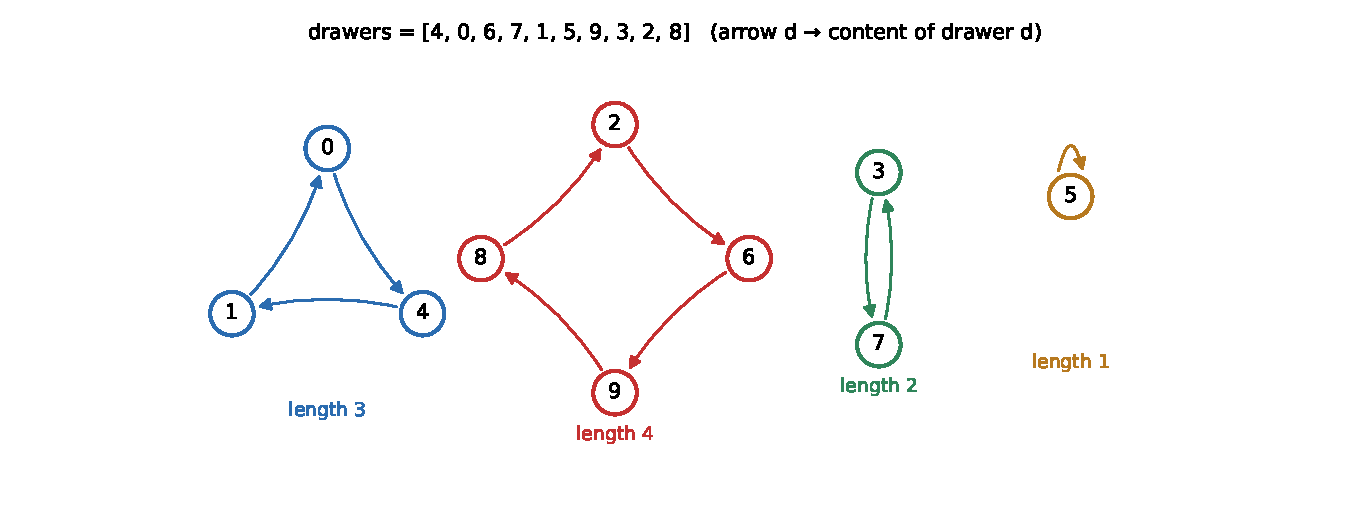
\includegraphics[width=0.8\linewidth]{figs/perm_cycles.pdf}\\
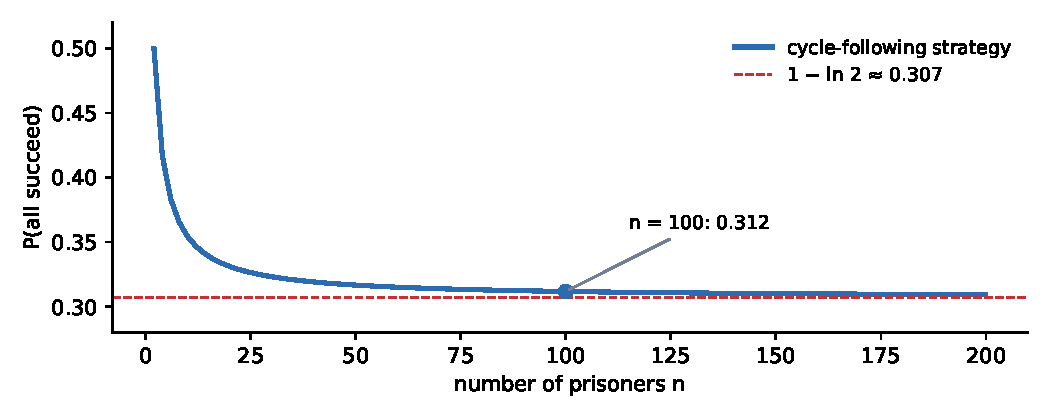
\includegraphics[width=0.62\linewidth]{figs/prisoners_prob.pdf}
\caption{\extra{} Cycles of a permutation ($n=10$) and $P(\text{win})$ as $n$ grows. Simulation with $10^5$ permutations (\texttt{--bin prisoners}): $0.3131$.}
\end{figure}


%======================================================================
\appendix
\section{From the professor's notes: is a binary tree a BST?}
Pages 7--8 of \texttt{SlidingWindowMaxima.pdf} contain a problem that is \textbf{not} in the recording of L3
(probably discussed at the end of L2, as a follow-up of the BST digression; check your L2 notes).
\profpage{0.55\linewidth}{7}{185bp}
\textbf{Wrong idea}: check only that for every node $v$, \texttt{v.left.key} $\le$ \texttt{v.key} $<$ \texttt{v.right.key}.
Counterexample in the notes: root $10$, left child $5$, whose right child is $12$: every local check passes, but $12$ is in the left subtree of $10$.
\profpage{0.55\linewidth}{8}{394bp}
\textbf{Correct recursion}: $P(v)$ returns (is it a BST?, min, max) of the subtree of $v$; \texttt{NULL} returns (true, $+\infty$, $-\infty$).
$v$ is a BST iff both children are and $M_\ell \le \texttt{v.key} < m_r$ (max of the left subtree, min of the right one).
One visit per node: $\Theta(n)$. \extra{} Rust version in \texttt{extra::is\_bst} (tested on the counterexample).
\end{document}
